\documentclass[titlepage,12pt]{article}
\usepackage[left=2.5cm, right=2.5cm, top=3.5cm, bottom=3.5cm]{geometry}
\usepackage[utf8]{inputenc}
\usepackage{listings}
\usepackage[all]{genealogytree}
\usepackage{enumitem}
\usepackage{amsmath}
\usepackage{csquotes}
\usepackage{url}
\usepackage[hidelinks]{hyperref}
\usepackage{float}
\hypersetup{
    colorlinks=false
}
\urlstyle{same}

\begin{document}

\title{ \Huge {\textbf{Infact}} \\[0.3in] \Large{A Social Media improved upon volunteer-based crowd sourced fact checking}}
\author{ Suraj Soni : 160050092 \\ Sai Teja Talluri : 160050098 \\ Chaithanya Naik : 160050102 \\ Jagadeep Sai : 160050104}
\date{$11^{th}$ October, 2018}
\maketitle

\tableofcontents

\newpage

\section{\textbf{Abstract}}
\paragraph{}
Mass social network platforms are highly prone to fallacious contents which can deteriorate the society. A good example of this could be the recent Whatsapp lynchings due to spread of provoking messages. We wish to create a platform which handles this problem using volunteer-based crowd sourcing.

\section{Broad Goal}
\paragraph{}
We would be creating a \textbf{web application} (\textit{and if time permits an app compatible with both android and iOS using flutter framework}) which would be a \textbf{social networking 
platform consisting of only articles as posts}. What makes this application unique is that the articles posted here are \textbf{fact checked by volunteers, with the help of centralized admins}.

\paragraph{}
The broad goal of this project is to create a platform to route the articles to be fact-checked to volunteer users in the backend and to make these articles available for Public 
(\textit{users other than volunteers and admins}) giving a flavour of social networking sites. This ensures the validity of the articles read by the users unlike any other platforms. 

\section{Functionalities}
\paragraph{}
Some of the major functionalities provided are as follows :
\begin{itemize}
    \item Different Login interfaces for Admin and Public. The volunteers will be among the public who have all the resources the general public has, plus they have special privileges to validate the articles. Any general public can become a volunteer by consent from the Admins.
    \item Route the articles acquired from a source to the appropriate volunteers based on their language expertise, genre of the articles they wish to review and their rating.
    \item After a volunteer does the fact checking and enters their conclusions, the result will be routed to other appropriate volunteers based on their rating for further checking with a constraint that who checks in late will get the further-checking task.
    \item If posts published has more negative response then it is stopped from circulation for verification and author is notified if possible to reevaluate and edit. 
    \item Rating system for volunteers based on their responses on the articles.True positive and true negative cases will increase their rating where as false negatives and false positives will a decrease.
    
    \item Users get the articles based on their selected preferences and also depending on the recently liked/read posts. They can also save their posts and view previously liked posts.
\end{itemize}

\section{Roles}
    \paragraph{}
    We have three different roles in total namely Admin, Volunteer and Public. Respective roles are as follows:
    \subsection{Admin}
    \begin{itemize}
    \setlength\itemsep{0.3em}
        \item Admins are the main source of articles to be crowd sourced by the volunteers.
        \item Admin can post articles and they will be given higher priority during verification \\ by the volunteers.
        \item Only admin has the power to recruit/fire volunteers and create new admins.
        \item Make decisions for articles with no proper orientation of correctness from volunteers
    \end{itemize}
    
    \subsection{Public}
    \begin{itemize}
     \setlength\itemsep{0.3em}
        \item Enjoy the verified content provided and can apply for volunteers (\textit{processed by admins})
        \item Can post articles themselves also.
    \end{itemize}
    
    \subsection{Volunteer}
    \begin{itemize}
     \setlength\itemsep{0.3em}
        \item Volunteer provides article verification and optionally comments possible edits to make the article correct.
        \item Upon correct verification their rating increases. But if rating drops down below a threshold they are fired and become normal users (Public).
    \end{itemize}
\section{Interfaces}
\paragraph{}
   We have divided the interfaces into two major categories namely Public/Volunteer and Admin interface. The brief description of the interfaces are as follows :
\subsection{Public/Volunteers}
\subsubsection{Log-in Interface}
\begin{itemize}
 \setlength\itemsep{0.3em}
    \item For login to their accounts by email. Users and Volunteers share the same login.
\item Has `Create Account` option for new Users. New Users will be asked their interested preferences for feed if any.
\end{itemize}
\subsubsection{Feed Related}
\begin{itemize}
 \setlength\itemsep{0.3em}
    \item Interface which list articles according to users interests, with option to \textit{save for later}.
	\item Interface to read the selected article and option to like or dislike the article
\end{itemize}
\subsubsection{Specifics}
\begin{itemize}
    \setlength\itemsep{0.3em}
    \item Details 
            \begin{itemize}
            \item Contains user details like email, phone number, feed preferences.
            \end{itemize}
    \item Post Related 
        \textit{ }
            \begin{itemize}
            \setlength\itemsep{0.3em}
            \item Interface to write articles and tag them to corresponding genres (sent to volunteers for verification)
            \item Interface to view the status of the published articles and comments why they weren't published, and option for edit and re-evaluate.
            
            \item Has three tabs each navigating to 
                \begin{itemize}
                    \setlength\itemsep{0.3em}
                    \item Posts posted, both pending posts and already published  (pending displayed above).
                    \item Posts liked.
                    \item Posts saved to view later.
                \end{itemize}
            
            \end{itemize}
\end{itemize}
\subsubsection{ Volunteer Related }
        \noindent
        \textit{ If User is also a volunteer : }
        \begin{itemize}
             \setlength\itemsep{0.3em}
            \item Interface where he sees a list of articles which he has to approve, where he can label articles as fallacious or correct, also comment on reasons for fallacy.
        \end{itemize}
        \noindent
        \textit{ If User's volunteer application is pending : }
        \begin{itemize}
            \item Interface to withdraw application.
        \end{itemize}
        \newpage
        \noindent
        \textit{ If User isn't a volunteer : }
        \begin{itemize}
             \setlength\itemsep{0.3em}
            \item Interface where the user can apply for volunteer, where he needs to fill additional details like qualification and expertise
        \end{itemize}
\subsection{Admin}
\begin{itemize}
     \setlength\itemsep{0.3em}
    \item Log-in Interface for admin 
    \item Interface for uploading articles
    \item  Interface to view responses and comments given by volunteers to the articles.
    \item Interface to select volunteers and make new admins
\end{itemize}
\subsection{ER Diagram}
\begin{figure}[H]
    \centering
    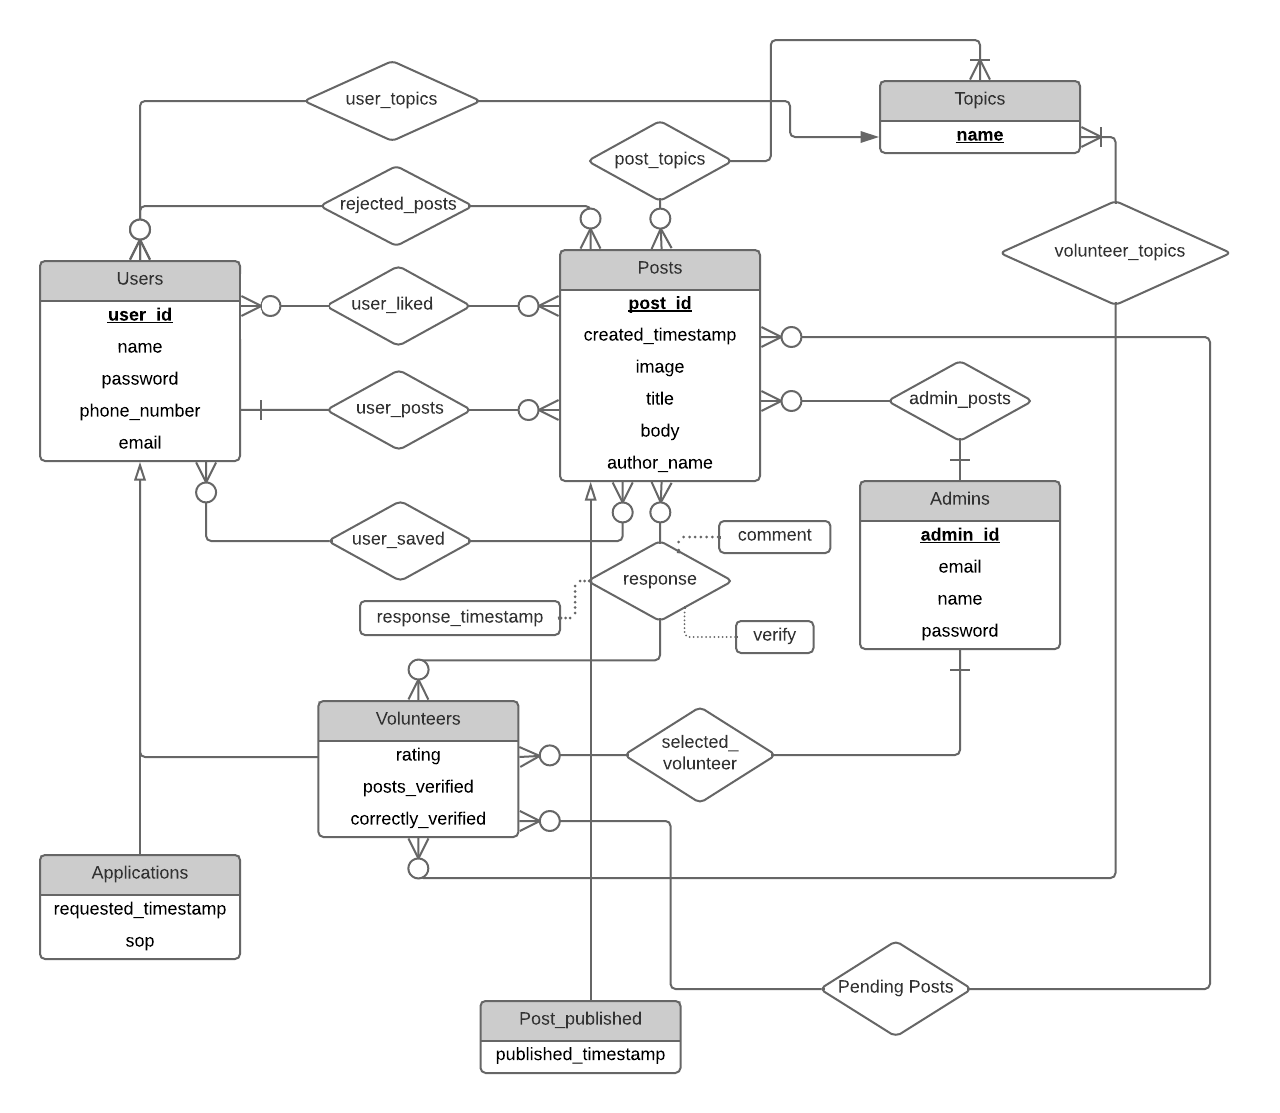
\includegraphics[width=1.1\textwidth]{EntityRelationshipDiagram}
    \caption{ER Diagram}
    \label{fig:er_diagram}
\end{figure}
\newpage
\subsection{Table Design}
\begin{figure}[H]
    \centering
    \includegraphics[width=1.1\textwidth]{Tabledesign.jpeg}
    \caption{Table design}
    \label{fig:table_design}
\end{figure}
\end{document}